\documentclass{article} 

\usepackage[english]{babel}
\usepackage[utf8]{inputenc}
\usepackage{fullpage}
\usepackage{amsmath}
\usepackage{graphicx}
\usepackage{float}
\usepackage[colorinlistoftodos]{todonotes}
\usepackage{hyperref}
\usepackage{amssymb}
\usepackage[utf8]{inputenc}
\usepackage[english]{babel}
% \usepackage{titlesec}
\usepackage[shortlabels]{enumitem}
 
\newtheorem{theorem}{Theorem}[section]
\newtheorem{corollary}{Corollary}[theorem]
\newtheorem{lemma}[theorem]{Lemma}
\setcounter{MaxMatrixCols}{20}


\usepackage{geometry}
 \geometry{
 a4paper,
 left=17.5mm,
 right=17.5mm,
 top=20mm,
 bottom=15mm
}

\title{227A Final Project}

\author{Boying Gong (SID: 24967354)}

\begin{document}

\twocolumn

\maketitle


% ========================= PART 1 =========================


\section{\textbf{Uncertainty Model}}

\subsection{AR Model Parameter Estimation}

\begin{enumerate}[A)]

\item \textbf{Formulation of the Optimization Problem}

    Denote the number of historical data as $n$ ($n=60$ in our case). We write the auto-regressive model in the matrix form (note that the model depends on the order $p$)
	\[
	\beta_p = \begin{pmatrix} 
		\beta(p+1)  \\
		\beta(p+2)  \\
		\vdots \\
		\beta(n) 
	\end{pmatrix},
	\theta_p = \begin{pmatrix} 
		\theta(1)  \\
		\vdots \\
		\theta(p) 
	\end{pmatrix},
    \epsilon_p = \begin{pmatrix} 
		\epsilon(p+1)  \\
		\epsilon(p+2)  \\
		\vdots \\
		\epsilon(n) 
	\end{pmatrix},
	\]
    \[
    H_p = \begin{pmatrix} 
        \beta(p)   & \beta(p-1) & \cdots & \beta(1)   \\
        \beta(p+1) & \beta(p)   & \cdots & \beta(2)   \\
        \vdots     & \vdots     & \ddots & \vdots     \\
        \beta(n-1) & \beta(n-2) & \cdots & \beta(n-p) \\
    \end{pmatrix}.
    \]
	\[ 
	\beta_p=H_p\theta_p+\sigma_p\epsilon_p, \quad ||\epsilon_p||_\infty \leq 1.
	\]

	Notive that the noice in the autoregressive model is assumed to be genrated based on infinity-norm constraint. Following the noice generation procedure, we estimate the values of $\theta_p$ and $\sigma_p$ by minimizing the infinity norm of the error
	\[
	\min_{\hat{\theta}_p}||\beta_p-\hat{\beta}_p||_\infty, \quad
    \text{s.t. }\hat{\beta}_p = H_p\hat{\theta}_p,
	\]
	This is equivalent to the following LP problem, where we use $\hat{\sigma}$ as an estimate of $\sigma$.
	\begin{equation}\label{eq:ar_opt} 
	\min_{\hat{\theta}_p, \hat{\sigma}_p}\hat{\sigma}_p, \quad
    \text{s.t. }\hat{\beta}_p=H_p\hat{\theta}_p,|\beta_p-\hat{\beta}_p|\preceq\hat{\sigma}_p.
	\end{equation}

\item\textbf{Order Selection for the AR Model}

    The order $p$ of the autoregressive model needs to be determined. Because our goal is to predict the cash flow requirement in the next 6 months, prediction error is important. We use cross-validation on a rolling basis to calculate the prediction error for $1\leq p\leq 30$. The cross-validation procedure is described as follows.\cite{cvTs} For each $p$, 
    \begin{enumerate}
    	\item Fit the model to the data $\beta_1,\cdots,\beta_t$ and let $\hat{\beta}^{(t)}_{t+1},\cdots,\hat{\beta}^{(t)}_{t+6}$ denote the forecasts of the next 6 months. Then compute the error ($e^{(t)}_{t+i} = \beta_{t+i}- \hat{\beta}^{(t)}_{t+i}$) for the forecast observations. 
        \item Repeat step 1 for $t=n-15,\cdots,n-6$ (10-fold). 
        \item Compute : (I) the proportion of absolute error $|e^{(t)}_{t+i}|$ that are greater than the $\sigma$ estimation $|\sigma^{(t)}|$. We call it out-of-bound error.
        (II) MAE (Mean Absolute Error) from the errors $e^{(t)}_{t+i}, t=n-15,\cdots,n-6,i=1,\cdots,6$. 
    \end{enumerate}
    Then, we choose $p$ with the smallest out-of-bound error. For $p$'s with the same out-of-bound error, we choose $p$ with the smallest MAE.

\item\textbf{Results}

     \begin{figure*}
        \centering
        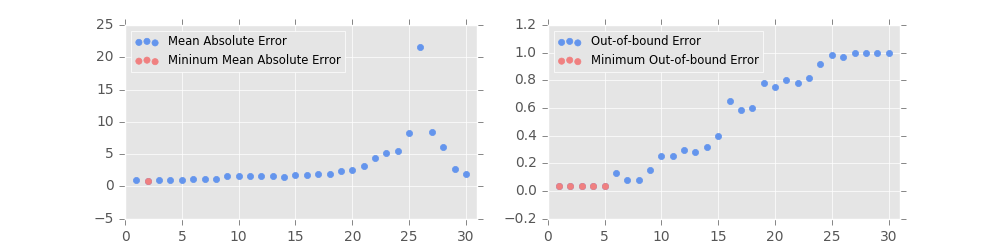
\includegraphics[width=0.7\textwidth]{cv.png}
        \caption{\emph{Cross-validation Results for order selection. Left: The cross-validation MAE for a variety of $p$'s. Right: The cross-validation out-of-bound error for a variety of $p$'s. The minimum error are marked red.}}
        \label{fig:cv_result}
    \end{figure*} 

    \begin{figure*}
        \centering
        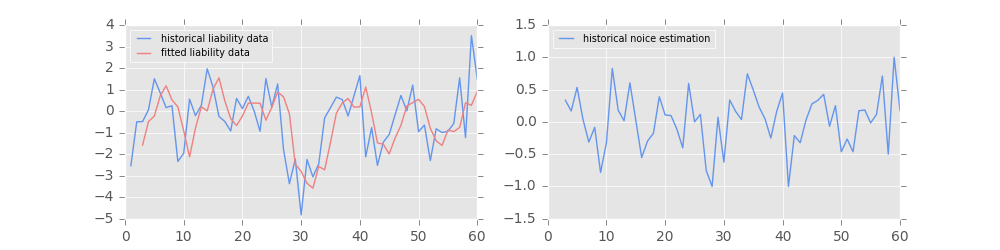
\includegraphics[width=0.7\textwidth]{uncertaintyModel.png}
        \caption{\emph{Visualation of fitted model. Left: The blue line show sthe historical liability data, and the red line shows the fitted value of our model using the order p = 2. Right: The blue line shows the estimation of historical noise $\hat{\sigma}$. Note that the actual prediction error will be multiplied by $\hat{\sigma}$.}}
        \label{fig:uncertaintyModel}
    \end{figure*} 

    The cross-validation results are shown in Figure \ref{fig:cv_result}, the minimum  out-of-bound error and MAE are both attained when $p=2$. We use $p=2$ to solve the optimization problem (\ref{eq:ar_opt}). The corresponding auto-regressive model is given by
    \begin{equation}\label{eq:ar-est}
        \beta(t+1) = \theta_1^*\beta(t) + \theta_2^*\beta(t-1)+\sigma^*\epsilon(t+1),
    \end{equation}
    \[\quad|\epsilon(t+1)|\leq 1.\]
    The solution for the 60 historical data is
    $\sigma^* = 3.243, \theta^*_1 = 0.449, \theta^*_2 = 0.533.$
    Notice that for the rolling-horizon based strategy, the above estimation will only used in January. In future months, the estimation will be updated given new liability data.

\end{enumerate}

\subsection{Uncertainty Model}

    Let $u = (\epsilon(t+1), \cdots, \epsilon(t+T))^T$. With the auto-regressive model (\ref{eq:ar-est}), $\hat{b}(t)$ and $B(t)$ can be expressed as a function of $\beta(t), \beta(t-1), \theta_1^*, \theta_2^*$ and $\sigma^*$ using recursive substitution. The derivation is given in Appendix \ref{apx:recursiveSubstitution}. From the historical data, $\beta(t) = 1.4880$ and $\beta(t-1)=3.5112$. The numerical value is given below
    \[
	   \hat{b}(t) = 
        \begin{pmatrix}
    	2.539 & 1.933 & 2.220 & 2.027 & 2.093 & 2.020
	   \end{pmatrix}^T,
    \]
    \[
	   B(t) = 
        \begin{pmatrix}
    	   3.243 & 0 & 0 & 0 & 0 & 0 \\
            1.456 & 3.243 & 0 & 0 & 0 & 0 \\
            2.382 & 1.456 & 3.243 & 0 & 0 & 0 \\
            1.846 & 2.382 & 1.456 & 3.243 & 0 & 0 \\
            2.098 & 1.846 & 2.382 & 1.456 & 3.243 & 0 \\
            1.925 & 2.098 & 1.846 & 2.382 & 1.456 & 3.243
        \end{pmatrix}.
    \]
    Similar to the AR model parameter, for the rolling-horizon based strategy, the above estimation will only used in January. In future months, the estimation will be updated with the updated AR model.


% ========================= PART 2 =========================

\section{\textbf{Decision Making}}

In this section, we provide the brief formulation of four strategies built in a rolling horizon fashion. They are: the naive strategy, the robust strategy, the rolling strategy and the relative robust strategy. We will show that the later three actually results in the same decision for rolling-horizon based implementation.

For a detailed problem formulation and variable definition, please refer to Appendix \ref{apx:problemFormulation}.

% ================== Naive Strategy ==================

\subsection{Naive Strategy}

    Let $C^{(1)}_{initial} = 70.3$ be the amount that the company has at the beginning of the horizon. We assume the future liability be $\hat{b}(t)$ without error.

    In January (i = 1), let $x^{(1)}=(x^{(1)}_{cash}, x^{(1)}_{cp}, x^{(1)}_{cre})$ be the decision variables $, x^{(1)}_{cash}\in\mathbb{R}^6, x^{(1)}_{cp}\in\mathbb{R}^3, x^{(1)}_{cre}\in\mathbb{R}^5$. We can write the optimization problem as follows.
    \begin{equation}
        \min_x c_1^Tx: A_1x+l_1\geq\hat{b}(t), 0\leq x\leq \bar{x}_1.
    \end{equation}
    where $l_1=\begin{pmatrix}C^{(1)}_{initial} & 0& 0& 0& 0& 0\end{pmatrix}^T$ represents the initial funds. Only the first of these decisions $x^{(1)}_{cre}(1)$, $x^{(1)}_{cp}(1)$ and $x^{(1)}_{cash}(1)$ will be implemented. Given the realization of the first month liability $\beta_1$, if the cash amount we reserved for liability is less than $\beta_1$, the strategy fails. If not, the extra part becomes the initial fund in February.

    In February ($i = 2$),  we re-estimate the AR model and the uncertainty model. The optimization problem for the second month is built on the updated parameters. And the number of decision variable is reduced by 3. That is, $x^{(2)}=(x^{(2)}_{cash}, x^{(2)}_{cp}, x^{(2)}_{cre}), x^{(2)}_{cash}\in\mathbb{R}^5, x^{(2)}_{cp}\in\mathbb{R}^2, x^{(2)}_{cre}\in\mathbb{R}^4$.

    Eventually, we will be solving six optimization problems sequentially, one for each month($i = 1, \cdots, 6$):
    \begin{equation}
        \min_x c_i^Tx: A_ix+l_i\geq\hat{b}(t+i-1), 0\leq x\leq \bar{x}_i.
    \end{equation}

% ================== Robust Strategy ==================

\subsection{Robust Strategy}

    Consider the robust counterpart of the naive strategy. Assume the liability vector is a function of uncertainty. In month $i$, the liability is a realization from the set $\mathcal{U}(t+i-1)$. For the rolling strategy, we will be solving the following optimization problems sequentially, one for each month($i = 1, \cdots, 6$):
    \begin{equation}\label{eq:robust}\begin{split}
        \min_x\ & c_i^Tx,\\
        \text{s.t. }& A_ix+l_i\geq b(t+i-1), \forall b(t+i-1)\in\mathcal{U}(t+i-1) ,\\
        & 0\leq x\leq \bar{x_i}.
    \end{split}\end{equation}
    They are equivalent to the following LP problems:
    \begin{equation}\label{eq:robust_final}\begin{split}
        \min_x\ & c_i^Tx,\\
        \text{s.t. }& A_ix+l_i\geq b(t+i-1)+|B(t+i-1)|\textbf{1} ,\\
        & 0\leq x\leq \bar{x_i}.
    \end{split}\end{equation}

% ========= Affine Strategy =========

\subsection{Affine Strategy}

    For the affine strategy, we assume that the decision variables are linear functions of previous information. we will be solving the following optimization problems sequentially ($i = 1, \cdots, 6$):
    \[\begin{split}
       \max_x\ & \min_{u:||u||_\infty \leq 1} c_i^Tx(u) \\
        \text{s.t. } & X_{cash},  X_{cp}, X_{cre} \text{ strictly lower-triangular,}\\
        & A_i(x + X_iu) + l_i\geq b(t+i-1),\forall b(t+i-1) \in \mathcal{U}(t+i-1) ,\\
        & 0\leq x+X_iu \leq \bar{x}_i.
    \end{split}\]
    They are equivalent to the following LP problems:
    \[\begin{split}
       \max_{x, X}\ & c_i^Tx - ||X^Tc_i||_1  \\
        \text{s.t. } & X_{cash},  X_{cp}, X_{cre} \text{ strictly lower-triangular,}\\
        & A_ix + l_i\geq  \hat{b}(t+i-1) + |B(t+i-1) - A_iX|\textbf{1}, \\
        & 0\leq x+Xu \leq \bar{x}_i.
    \end{split}\]   

    \begin{figure*}
        \label{fig:regret}
        \begin{minipage}{0.5\textwidth}
            \centering  
            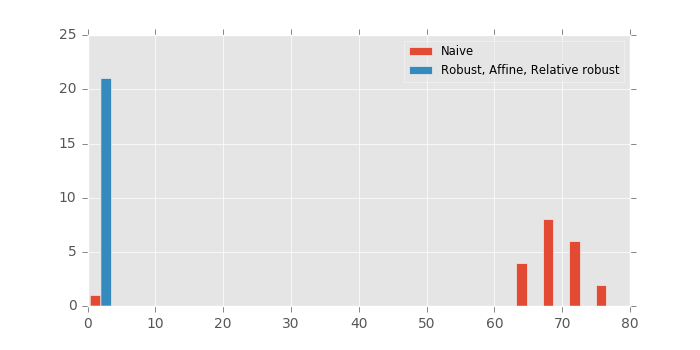
\includegraphics[width=\textwidth]{rolling_regret.png}
        \end{minipage}
        \begin{minipage}{0.5\textwidth}
            \centering  
            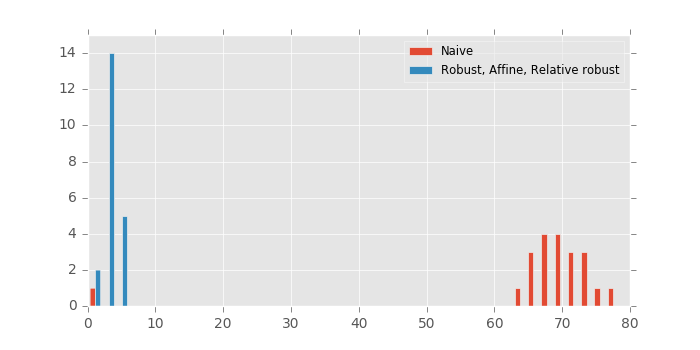
\includegraphics[width=\textwidth]{regret.png}
        \end{minipage}
        \caption{\emph{Left: The regret histogram for rolling strategy. Right: the regret histogram for non-rolling strategy.}}
    \end{figure*}

    \begin{table*}
        \label{table:regret}
        \centering
        \begin{tabular}{l|p{1.3cm}|p{1.3cm}|p{1.3cm}|p{1.3cm}|p{1.3cm}|p{1.3cm}|p{1.3cm}|p{1.3cm}|}
        \cline{2-9}
        & \multicolumn{4}{|c|}{Rolling strategy} & \multicolumn{4}{|c|}{Non-rolling strategy} \\
        \cline{2-9}
        & Naive & Robust & Affine & Relative Robust & Naive & Robust & Affine & Relative Robust \\ 
        \hline
        \multicolumn{1}{|c|}{Fail Percentage}  & 95.2\% & 0\% & 0\% & 0\% & 33.3\% & 0\% & 0\% & 0\%\\
        \hline
        \end{tabular}
        \caption{\emph{Percentage of bankrutcy (could not meet the liability) for rolling-based and non-rolling-based version of the four strategies.}}
    \end{table*}

% ========= Relative Robust Strategy =========

\subsection{Relative Robust Strategy}

    For the relative robust strategy, we consider minimizing the maximum regret for problem (\ref{eq:robust}). For now, we first consider the problem without rolling, and omit the month subscripts for simplicity. We will prove that the relative robust strategy is actually equivalent to the robust strategy.

    The regret function measures the difference between the performance of the solution with and without the full knowledge of the future. Assume we choose $x$ as decision vector, $u$ is the vector of realized parameter values and $x^*(u)$ is the optimal decision vector if $u$ is available. The regret associated with having chosen $x$ rather than $x^*(u)$ as decision vector is defined as follows,
    \[
        r(x, u) =  c^Tx - c^Tx^*(u).
    \]
    The regret will always be greater than 0. The relative robust problem of minimizing the maximum regret can be formulated as follows
    \[\begin{split}
        \min_{x} & \big\{ \quad\max_{||u||_\infty\leq 1} \big\{c^Tx - 
        \min_{\{y:Ay+l\geq \hat{b}(t)+B(t)u, 0\leq y\leq \bar{x} \}} c^Ty\big\}\big\}. \\
        \text{s.t. } & Ax+l\geq \hat{b}(t) + B(t)u, \forall ||u||_\infty\leq 1, \\
        & 0\leq x\leq \bar{x}.
    \end{split}\]
    Introducing a slack variable $\gamma$ that expresses an upper bound on the regret, we can equivalently reformulate this problem as follows,
    \[\begin{split}
        \min_{x, y, \gamma}\ & \gamma \\
        \text{s.t. } 
        & Ax+l\geq \hat{b}(t) + B(t)u, \forall ||u||_\infty\leq 1,  \\
        & 0\leq x\leq \bar{x}, \\
        & \gamma \geq c^Tx + \max_{||u||_\infty\leq 1} \big\{
        \max_{\{y:Ay+l\geq \hat{b}(t)+B(t)u, 0\leq y\leq \bar{x} \}} - c^Ty\big\}.
    \end{split}\]
    Similar to the robust problem and the affine problem, this can also be expressed as{} follows
    \begin{equation}\label{eq:relative}\begin{split}
        \min_{x, y, \gamma}\ & \gamma \\
        \text{s.t. } 
        & Ax+l\geq \hat{b}(t) + |B(t)|\textbf{1}, \\
        & 0\leq x\leq \bar{x}, \\
        & \gamma \geq c^Tx + \max_{||u||_\infty\leq 1} \big\{
        \max_{\{y:Ay+l\geq \hat{b}(t)+B(t)u, 0\leq y\leq \bar{x} \}} - c^Ty\big\}.
    \end{split}\end{equation}
    Notice that the set $\{||u||_\infty \leq 1\}$ can be expressed as a convex hull of a finite number of extreme scenarios, namely
    \[\{||u||_\infty \leq 1\} = \text{conv}(\{u^{[i]}, i = 1, \cdots, 2^T\})\]
    We have the following lemma:

    \begin{lemma}
        The following are equivalent, 
        \begin{enumerate}
            \item $-c^Tx+\gamma \geq
            \max_{\{y:Ay+l\geq \hat{b}(t)+B(t)u, 0\leq y\leq \bar{x} \}} - c^Ty,$\\ $\forall ||u||_\infty\leq 1,$
            \item $-c^Tx+\gamma \geq
            \max_{\{y:Ay+l\geq \hat{b}(t)+B(t)u^{[i]}, 0\leq y\leq \bar{x} \}} - c^Ty,$\\$ i = 1, \cdots, 2^T$.
        \end{enumerate}
    \end{lemma}
    \emph{Proof. } For the proof, please refer to Corollary 4.1 in \cite{hauser2013relative}.

    Thus, problem (\ref{eq:relative}) is equivalent to 
    \begin{equation}\label{eq:relative_final}\begin{split}
        \min_{x, y, \gamma}\ & \gamma \\
        \text{s.t. } 
        & Ax+l\geq \hat{b}(t) + |B(t)|\textbf{1}, \\
        & 0\leq x\leq \bar{x}, \\
        & \gamma \geq c^Tx + g(i),  i = 1, \cdots, 2^T, \\
        & g(i) = \max_{\{y:Ay+l\geq \hat{b}(t)+B(t)u^{[i]}, 0\leq y\leq \bar{x} \}} - c^Ty.
    \end{split}\end{equation}

    We can solve problem (\ref{eq:relative_final}) with a two-step procedure where we first solve an LP problem for $y$ (that is, solve $g(i)$), and then solve the LP problem for $x$ and $\gamma$.

    Notice that the optimal solution of (\ref{eq:relative}) is equal to the optimal solution of the robust problem (\ref{eq:robust_final}). To see this fact, let $g = \max_i g(i)$. $g$ can be treated as a constant since $g(i)$ can be solved explicitly. Then (\ref{eq:relative}) is equivalent to the following
    \[\begin{split}
        \min_{x, y}\ & c^Tx + g \\
        \text{s.t. } 
        & Ax+l\geq \hat{b}(t) + |B(t)|\textbf{1}, \\
        & 0\leq x\leq \bar{x}.
    \end{split}\]
    which is the same as (\ref{eq:robust_final}). Note that the robust solution and relative robust optimization problem does not usually equivalent to each other without the infinity norm assumption and the linearity of objective and constraints function.

% ========================= PART 3 =========================

\section{Initial Fund Analysis}

Please see appendix \ref{apx:InitialFundAnalysis}.

\section{\textbf{Evaluation Metrics}}

    We now use the notion of regret to compare different strategies. We implemented the rolling-based and non-rolling-based version of the four strategies described in the last section. Recall the definition of regret in the last section:
    \[
        r(x, u) =  c^Tx - c^Tx^*(u).
    \]
    In the case where the strategy fails to meet the required liabilities, we let $c^Tx^*(u)$ be zero such that the reget is large.

    Figure \ref{fig:regret} and Table \ref{table:regret} shows that the robust, affine and relative robust strategy have every small probability of bankruptcy ($\sim$ 0). The rolling naive strategy is very likely to fail. And the bankruptcy probability of non-rolling naive strategy is much lower than its rolling counterpart. 

    In contrast to the high regret of the non-rolling strategy for the robust problems, the rolling version of the robust, affine and relative robust strategy generally result in much smaller regret with the mean regret being around 3. 

    Thus, we would recommend using the rolling version of the robust, affine and relative robust strategy (which are equivalent to each other) for the cash-flow management problem in order to minimize the regret.


\bibliographystyle{plain}
\bibliography{Proof_of_Correctness.bib}

\clearpage
\newpage
\appendix

\onecolumn

% ======================= Appendix A =======================


\section{Optimization Problem Formulation}\label{apx:problemFormulation}

\subsection{Naive Strategy}

    Let $C^{(1)}_{initial} = 70.3$ be the amount that the company has at the beginning of the horizon. We assume the future liability be $\hat{b}(t)$ without error. We now describe the rolling-horizon naive strategy.
    
    In January ($i = 1$), let $x^{(1)}=(x^{(1)}_{cash}, x^{(1)}_{cp}, x^{(1)}_{cre})$ be the decision variables $, x^{(1)}_{cash}\in\mathbb{R}^6, x^{(1)}_{cp}\in\mathbb{R}^3, x^{(1)}_{cre}\in\mathbb{R}^5$. The company can draw an amount $x^{(1)}_{cre}(1)$ from its line of credit and issue an amount $x^{(1)}_{cp}(1)$ of commercial paper. Together with the initial asset $C^{(1)}_{initial}$, $x^{(1)}_{cre}(1)+x^{(1)}_{cp}(1)+C^{(1)}_{initial}$ will be used for investment and meeting the liabilities. The balance equation is as follows, 
    \[
        x^{(1)}_{cre}(1)+x^{(1)}_{cp}(1)+C^{(1)}_{initial}\geq x^{(1)}_{cash}(1) + \hat{b}_1(t).
    \]
    Similarly, we can get the equation for other months and obtain the following LP formulation:
    \[
        \begin{split}
            \max_{x} \quad & x^{(1)}_{cash}(6) \\
            \text{s.t.} \quad 
            & x^{(1)}_{cre}(1) + x^{(1)}_{cp}(1)+C^{(1)}_{initial}-x^{(1)}_{cash}(1) \geq \hat{b}_1(t), \\
            & x^{(1)}_{cre}(2) + x^{(1)}_{cp}(2) -1.01x^{(1)}_{cre}(1) + 1.003x_{cash}(1) -x^{(1)}_{cash}(2) \geq \hat{b}_2(t),  \\
            & x^{(1)}_{cre}(3) + x^{(1)}_{cp}(3) -1.01x^{(1)}_{cre}(2) + 1.003x_{cash}(2) -x^{(1)}_{cash}(3) \geq \hat{b}_3(t),  \\
            & x^{(1)}_{cre}(4) - 1.02x^{(1)}_{cp}(1) - 1.01x^{(1)}_{cre}(3) + 1.003x_{cash}(3) - x^{(1)}_{cash}(4) \geq \hat{b}_4(t),  \\
            & x^{(1)}_{cre}(5) - 1.02x^{(1)}_{cp}(2) - 1.01x^{(1)}_{cre}(4) + 1.003x_{cash}(4) - x^{(1)}_{cash}(5) \geq \hat{b}_5(t),  \\
            & - 1.02x^{(1)}_{cp}(3) - 1.01x^{(1)}_{cre}(5) + 1.003x^{(1)}_{cash}(5) - x^{(1)}_{cash}(6) \geq \hat{b}_6(t),  \\
            & 0 \leq x^{(1)}_{cre}(i) \leq 1, i = 1, \cdots, 5.\\
            & x^{(1)}_{cp} \geq 0, i = 1, 2, 3.\\
            & x^{(1)}_{cash}(i)\geq 0, i = 1, \cdots, 6.
        \end{split}
    \]
    Write this in LP format:
    \begin{equation}\label{eq:naiveJan}
        \min_x c_1^Tx: A_1x+l_1\geq\hat{b}(t), 0\leq x\leq \bar{x}_1.
    \end{equation}
    where $l_1 = \begin{pmatrix}C^{(1)}_{initial} & 0& 0& 0& 0& 0\end{pmatrix}^T$ and 
    \[
        A_1
        = 
        \begin{pmatrix}
            a_1^T \\
            a_2^T \\
            a_3^T \\
            a_4^T \\
            a_5^T \\
            a_6^T
        \end{pmatrix}
        =
        \begin{pmatrix}
            -1    &   0    &   0    &  0    &  0    &  0    &  1    &  0   &  0   &  1     &   0   &  0   &  0   &  0   \\
            1.003 &  -1    &   0    &  0    &  0    &  0    &  0    &  1   &  0   &  -1.01 &   1   &  0   &  0   &  0   \\
            0     & 1.003  &   -1   &  0    &  0    &  0    &  0    &  0   &  1   &  0     & -1.01 &  1   &  0   &  0   \\
            0     &  0     & 1.003  &   -1  &  0    &  0    & -1.02 &  0   &  0   &  0     &  0    & -1.01&  1   &  0   \\
            0     &  0     &  0     & 1.003 &  -1   &  0    &  0    &-1.02 &  0   &  0     &  0    &  0   &-1.01 &  1   \\
            0     &  0     &  0     &  0    & 1.003 &  -1   &  0    &  0   &-1.02 &  0     &  0    &  0   &  0   &-1.01
        \end{pmatrix}.
    \]

    After solving the optimization problem (\ref{eq:naiveJan}), only the first of these decisions $x^{(1)}_{cre}(1)$, $x^{(1)}_{cp}(1)$ and $x^{(1)}_{cash}(1)$ will be implemented. 

    Assume the realization of the liability of January is $\beta_1$. If $x^{(1)}_{cre}(1)+x^{(1)}_{cp}(1)+C^{(1)}_{initial} - x^{(1)}_{cash}(1) \leq \beta_1$, the company will not be able to meet the required liability, and the strategy would fail. If $x^{(1)}_{cre}(1)+x^{(1)}_{cp}(1)+C^{(1)}_{initial} - x^{(1)}_{cash}(1) \geq \beta_1$, the company will have $C^{(2)}_{initial} =  x^{(1)}_{cre}(1)+x^{(1)}_{cp}(1)+C^{(1)}_{initial} - x^{(1)}_{cash}(1) - \beta_1$ at the beginning of Feburary. Moreover, we can use $\beta_1$ to get the updated uncertainty model $\hat{b}(t+1)\in\mathbb{R}^5$ and $B(t+1)\in\mathbb{R}^{5\times5}$.

    In Feburary ($i = 2$), let $x^{(2)}=(x^{(2)}_{cash}, x^{(2)}_{cp}, x^{(2)}_{cre})$ be the decision variables, $x^{(2)}_{cash}\in\mathbb{R}^5, x^{(2)}_{cp}\in\mathbb{R}^2, x^{(2)}_{cre}\in\mathbb{R}^4$. The company can draw an amount $x^{(2)}_{cre}(2)$ from its line of credit and issue an amount $x^{(2)}_{cp}(2)$ of commercial paper. In addition, principal plus interest of $1.01x^{(1)}_{cre}(1)$ is due on the line of credit and $1.003x^{(1)}_{cash}(1)$ is received on the invested excess funds. Thus, $1.003x^{(1)}_{cash}(1)+x^{(2)}_{cre}(2)+x^{(2)}_{cp}(2)+C^{(2)}_{initial}$ will be used for investment, meeting the liabilities and payment of credit line. The balance equation is as follows, 
        \[
            1.003x^{(1)}_{cash}(1)+x^{(2)}_{cre}(2)+x^{(2)}_{cp}(2)+C^{(2)}_{initial}\geq x^{(2)}_{cash}(2) + \hat{b}_2(t+1)+1.01x^{(2)}_{cre}(1).
        \]
    The equation for other months are the same as January. We can obtain the following LP fomulation:
    \begin{equation}\label{eq:naiveFeb}
        \min_x c_2^Tx: A_2x+l_2\geq\hat{b}(t+1), 0\leq x\leq \bar{x}_2.
    \end{equation}
    where $l_2 = \begin{pmatrix}C^{(2)}_{initial} & 0& 0& 0& 0\end{pmatrix}^T$.

    Similarly, only $x^{(2)}_{cre}(2)$, $x^{(2)}_{cp}(2), x^{(2)}_{cash}(2)$ will be implemented. We can then solve similar problems in the following months and obtain the decision variables. Finally in June(i = 6), there is only one decision variable $x^{(6)}_{cash}(6)$, and we need to solve the following problem:
    \[
        \begin{split}
            \max_{x} \quad & x^{(6)}_{cash}(6) \\
            \text{s.t.} \quad 
            & - 1.02x^{(3)}_{cp}(3) - 1.01x^{(5)}_{cre}(5) + 1.003x^{(5)}_{cash}(5) - x^{(6)}_{cash}(6) \geq \hat{b}_6(t+5),  \\
            & x^{(6)}_{cash}(6)\geq 0
        \end{split}
    \]
    Or equivalently,
    \begin{equation}\label{eq:naiveJune}
        \min_x c_6^Tx: A_6x+l_6\geq\hat{b}(t+5), 0\leq x\leq \bar{x}_5.
    \end{equation}
    If feasible, this problem is trivial with optimal solution being $x^{(6)}_{cash}(6) = - 1.02x^{(3)}_{cp}(3) - 1.01x^{(5)}_{cre}(5) + 1.003x^{(5)}_{cash}(5) - \hat{b}_6(t+5)$. The final cash amount in the end of June is 
    \[- 1.02x^{(3)}_{cp}(3) - 1.01x^{(5)}_{cre}(5) + 1.003x^{(5)}_{cash}(5) - \beta_6.\]

    Notice that the above procedure is equivalent solving six optimizaiton problems sequentially, one for each month($i = 1, \cdots, 6$):
    \begin{equation}\label{naiveAll}
        \min_x c_i^Tx: A_ix+l_i\geq\hat{b}(t+i-1), 0\leq x\leq \bar{x}_i.
    \end{equation}

\section{Robust Strategy}

    Consider the robust counterpart of the naive strategy (\ref{naiveAll}). Assume the liability vector is a function of uncertainty. In month $i$, the liability is a realization from the set $\mathcal{U}(t+i-1)$. For the rolling strategy, we will be solving the following optimizaiton problems sequentially, one for each month($i = 1, \cdots, 6$):
    \begin{equation}\label{eq:robust}
       \min_x c_i^Tx: A_ix+l_i\geq b(t+i-1), b(t)\in\mathcal{U}(t+i-1) ,0\leq x\leq \bar{x}_i
    \end{equation}
    The constrains $A_ix+l_i\geq b(t+i-1), b(t)\in\mathcal{U}(t+i-1)$ can be written as follows based on the autoregressive model assumption
    \[\begin{split}
        & A_ix+l_i\geq b(t+i-1), b(t)\in\mathcal{U}(t+i-1), \forall ||u||_\infty \leq 1 \\
        \iff & A_ix+l_i\geq b(t+i-1) + \max_{||u||_\infty \leq 1}B(t+i-1)u \\
        \iff & A_ix+l_i\geq b(t+i-1) + |B(t+i-1)|\textbf{1}
    \end{split}\]
    Thus, we can formulate the model as
    \begin{equation}\label{eq:robust_final}
        \min_x c_i^Tx: A_ix+l_i\geq b(t+i-1)+|B(t+i-1)|\textbf{1}, 0\leq x\leq \bar{x_i}.
    \end{equation}

\section{Affine Strategy}

    We now omit the month subcripts for simplicity. Assume that at each time $t$, the information in previous time points (up to $t-1$) are available. We further assume that the decision variables are linear functions of previous information.
    \[
        x_{cash}(u) = x_{cash} + X_{cash}u,
    \]
    \[ 
        x_{cp}(u) = x_{cp} + X_{cp}u,
    \]
    \[ 
        x_{cre}(u) = x_{cre} + X_{cre}u.
    \]
    Let $X=(X_{cash}^T, X_{cp}^T, X_{cre}^T)^T$, the optimization problem can be formulated as 
    \[\begin{split}
       \max_x\ & \min_{u:||u||_\infty \leq 1} c^Tx(u) \\
        \text{s.t. } & X_{cash},  X_{cp}, X_{cre} \text{ strictly lower-triangular,}\\
        & A(x + Xu) + l\geq b(t) + B(t)u,\forall b(t) \in \mathcal{U},\\
        & 0\leq x+Xu \leq \bar{x}.
    \end{split}\]
    The constraint $A(x + Xu) + l\geq b(t) + B(t)u,\forall b(t) \in \mathcal{U}$ can be written as follows
    \[\begin{split}
        & A(x + Xu) + l\geq \hat{b}(t) + B(t)u,\forall ||u||_\infty\leq 1 \\
        \iff & Ax+l\geq \hat{b}(t) + (B(t)-AX)u, \forall ||u||_\infty \leq 1 \\
        \iff & Ax+l\geq \hat{b}(t) + \max_{||u||_\infty \leq 1}(B(t)-AX)u \\
        \iff & Ax+l\geq \hat{b}(t) + |(B(t)-AX)|\textbf{1}
    \end{split}\]
    The objective function $\min_{u:||u||_\infty \leq 1} c^Tx(u)$ is equivalent to
    \[\begin{split}
    & c^Tx - \max_{u:||u||_\infty \leq 1} c^TX(-u) \\
    = & c^Tx - ||X^Tc||_1
    \end{split}\]
    Thus, we can formulate the affine strategy as the following LP problem
    \[\begin{split}
       \max_{x, X}\ & c^Tx - ||X^Tc||_1  \\
        \text{s.t. } & X_{cash},  X_{cp}, X_{cre} \text{ strictly lower-triangular,}\\
        & Ax + l\geq  \hat{b}(t) + |B(t) - AX|\textbf{1}, 0\leq x+Xu \leq \bar{x}.
    \end{split}\]






% ======================= Appendix B =======================


\section{Initial Fund Analysis}\label{apx:InitialFundAnalysis}

For simplicity, we only discuss how initial fund will influence the non-rolling strategy. The anlaysis for the rolling strategy will be similar.

Figure \ref{fig:naive}, \ref{fig:robust} and \ref{fig:affine} show that if the company have sufficient amount of initial asset, say 70.3 million, the naive strategy and the robust strategy will not turn to credit line nor commercial paper. As we decrease the amount of initial funds, the optimal amount for credit line $X_{cre}$ and commercial paper $X_{cp}$ will stay 0. The optimal value of excess funds to be invested $X_{cash}$ will decrease linearly. This is because it is the only source to cover the liability and the constraints are linear. When the initial funds drops below a thredhold (12.739 million for naive strategy and 60.2 million for robust and affine strategy), the problem will become infeasible.

    \begin{figure}[H]
       \centering
       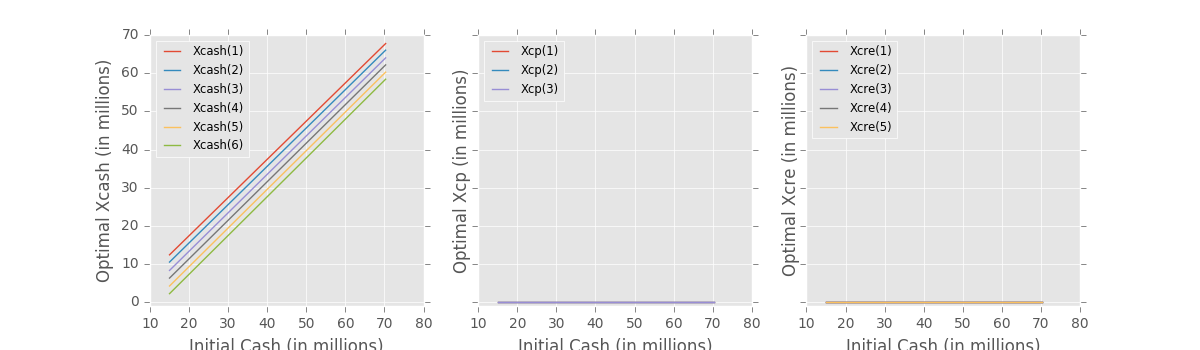
\includegraphics[width=0.7\textwidth]{naive.png}
        \caption{Optimal naive strategy for difference initial assets}
        \label{fig:naive}
    \end{figure}  

    \begin{figure}[H]
       \centering
       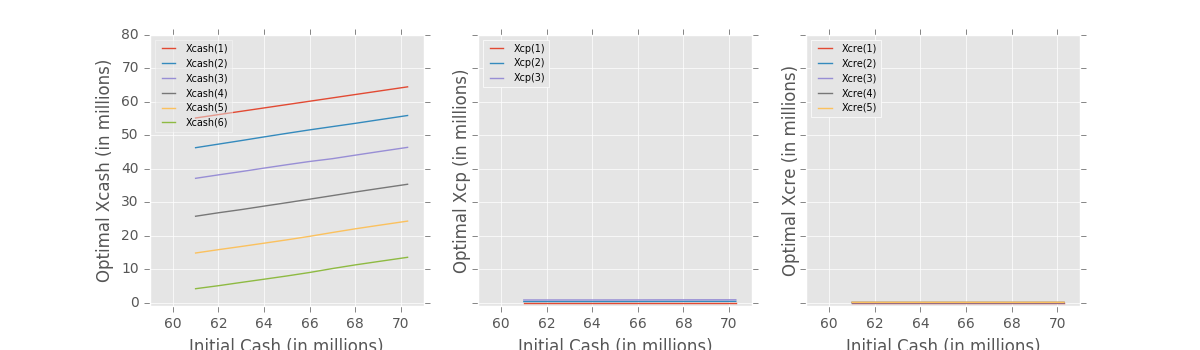
\includegraphics[width=0.7\textwidth]{robust.png}
        \caption{Optimal robust strategy for difference initial assets}
        \label{fig:robust}
    \end{figure}  

    \begin{figure}[H]
       \centering
       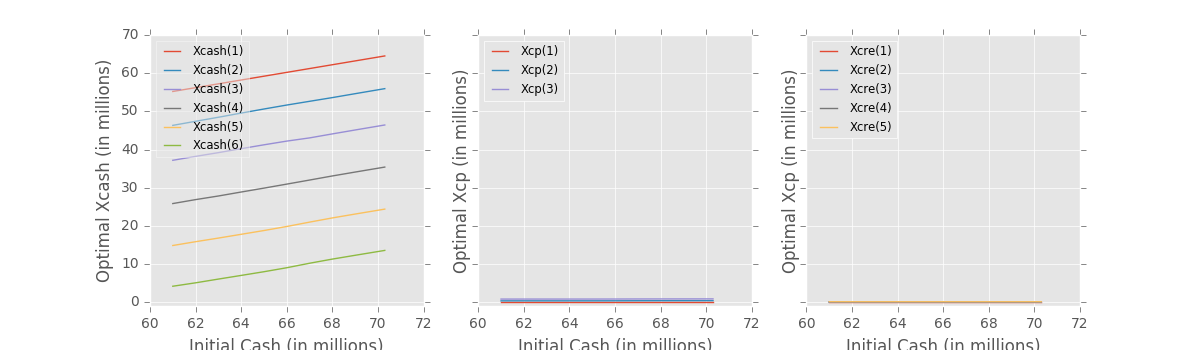
\includegraphics[width=0.7\textwidth]{affine.png}
        \caption{Optimal affine strategy for difference initial assets}
        \label{fig:affine}
    \end{figure}


% ======================= Appendix C =======================


\section{Appendix: AR(2) Recursive Substitution}\label{apx:recursiveSubstitution}

    Let $u = (\epsilon(t+1), \cdots, \epsilon(t+T))^T$. With the auto-regressive model (\ref{eq:ar-est}), $\hat{b}(t)$ and $B(t)$ can be expressed as a function of $\beta(t), \beta(t-1), \theta_1^*, \theta_2^*$ and $\sigma^*$ using recursive substitution. 
    \[\beta(t+1) = \theta_1\beta(t)+\theta_2\beta(t-1)+\sigma\epsilon(t+1)\]
    \[\begin{split}
        \beta(t+2) 
        = & \theta_1\beta(t+1)+\theta_2\beta(t)+\sigma\epsilon(t+2) \\
        = & \theta_1[\theta_1\beta(t)+\theta_2\beta(t-1)+\sigma\epsilon(t+1)]+
            \theta_2\beta(t)+\sigma\epsilon(t+2) \\
        = & (\theta_1^2+\theta_2)\beta(t)+\theta_1\theta_2\beta(t-1)+
            \theta_1\sigma\epsilon(t+1)+\sigma\epsilon(t+2)
    \end{split}\]
    \[\begin{split}
        \beta(t+3) 
        = & \theta_1\beta(t+2)+\theta_2\beta(t+1)+\sigma\epsilon(t+3) \\
        = & \theta_1\big[(\theta_1^2+\theta_2)\beta(t)+\theta_1\theta_2\beta(t-1)+
            \theta_1\sigma\epsilon(t+1)+\sigma\epsilon(t+2)\big]+ \\
          & \theta_2\big[\theta_1\beta(t)+\theta_2\beta(t-1)+\sigma\epsilon(t+1)\big]+\sigma\epsilon(t+3) \\
        = & (\theta_1^3+2\theta_1\theta_2)\beta(t) + (\theta_1^2\theta_2+\theta_2^2)\beta(t-1) + \\
          & (\theta_1^2+\theta_2)\sigma\epsilon(t+1) + \theta_1\sigma\epsilon(t+2) +
            \sigma\epsilon(t+3)
    \end{split}\]
    \[\begin{split}
        \beta(t+4) 
        = & \theta_1\beta(t+3)+\theta_2\beta(t+2)+\sigma\epsilon(t+4) \\
        = & \theta_1\big[ (\theta_1^3+2\theta_1\theta_2)\beta(t) + (\theta_1^2\theta_2+\theta_2^2)\beta(t-1) + \\
          & (\theta_1^2+\theta_2)\sigma\epsilon(t+1) + \theta_1\sigma\epsilon(t+2) +
            \sigma\epsilon(t+3)\big]+\\
          & \theta_2\big[ (\theta_1^2+\theta_2)\beta(t)+\theta_1\theta_2\beta(t-1)+
            \theta_1\sigma\epsilon(t+1)+\sigma\epsilon(t+2)\big]+\sigma\epsilon(t+4) \\
        = & (\theta_1^4+3\theta_1^2\theta_2+\theta_2^2)\beta(t)+
            (\theta_1^3\theta_2+2\theta_1\theta_2^2)\beta(t-1)+\\
           & (\theta_1^3+2\theta_1\theta_2)\sigma\epsilon(t+1)+(\theta_1^2+\theta_2)\sigma\epsilon(t+2)+\theta_1\sigma\epsilon(t+3)+\sigma\epsilon(t+4)
    \end{split}\]
    \[\begin{split}
        \beta(t+5) = & \theta_1\beta(t+4)+\theta_2\beta(t+3)+\sigma\epsilon(t+5) \\
        = & \theta_1\big[(\theta_1^4+3\theta_1^2\theta_2+\theta_2^2)\beta(t)+
            (\theta_1^3\theta_2+2\theta_1\theta_2^2)\beta(t-1)+\\
          & (\theta_1^3+2\theta_1\theta_2)\sigma\epsilon(t+1)+(\theta_1^2+\theta_2)\sigma\epsilon(t+2)+\theta_1\sigma\epsilon(t+3)+\sigma\epsilon(t+4)\big]+\\
          & \theta_2\big[(\theta_1^3+2\theta_1\theta_2)\beta(t) + (\theta_1^2\theta_2+\theta_2^2)\beta(t-1) + \\
          & (\theta_1^2+\theta_2)\sigma\epsilon(t+1) + \theta_1\sigma\epsilon(t+2) +
            \sigma\epsilon(t+3)\big]+\sigma\epsilon(t+5) \\
        = & (\theta_1^5+4\theta_1^3\theta_2+3\theta_1\theta_2^2)\beta(t) +
            (\theta_1^4\theta_2+3\theta_1^2\theta_2^2+\theta_2^3)\beta(t-1) + \\
          &(\theta_1^4+3\theta_1^2\theta_2+\theta_2^2)\sigma\epsilon(t+1)+(\theta_1^3+2\theta_1\theta_2)\sigma\epsilon(t+2)+(\theta_1^2+\theta_2)\sigma\epsilon(t+3)+\theta_1\sigma\epsilon(t+4)+\sigma\epsilon(t+5)
    \end{split}\]
    \[\begin{split}
        \beta(t+6) =
          & \theta_1\beta(t+5)+\theta_2\beta(t+4)+\sigma\epsilon(t+6) \\
        = & \theta_1\big[(\theta_1^5+4\theta_1^3\theta_2+3\theta_1\theta_2^2)\beta(t) +
            (\theta_1^4\theta_2+3\theta_1^2\theta_2^2+\theta_2^3)\beta(t-1)\\
          & (\theta_1^4+3\theta_1^2\theta_2+\theta_2^2)\sigma\epsilon(t+1)+(\theta_1^3+2\theta_1\theta_2)\sigma\epsilon(t+2)+(\theta_1^2+\theta_2)\sigma\epsilon(t+3)+\theta_1\sigma\epsilon(t+4)+\sigma\epsilon(t+5)\big]+\\
          & \theta_2\big[(\theta_1^4+3\theta_1^2\theta_2+\theta_2^2)\beta(t)+
            (\theta_1^3\theta_2+2\theta_1\theta_2^2)\beta(t-1)+\\
          & (\theta_1^3+2\theta_1\theta_2)\sigma\epsilon(t+1)+(\theta_1^2+\theta_2)\sigma\epsilon(t+2)+\theta_1\sigma\epsilon(t+3)+\sigma\epsilon(t+4)\big]+\sigma\epsilon(t+6) \\
        = & (\theta_1^6+5\theta_1^4\theta_2+6\theta_1^2\theta_2^2+\theta_2^3)\beta(t) +
            (\theta_1^5\theta_2+4\theta_1^3\theta_2^2+3\theta_1\theta_2^3)\beta(t-1)\\
          & (\theta_1^5+4\theta_1^3\theta_2+3\theta_1\theta_2^2)\sigma\epsilon(t+1)+(\theta_1^4+3\theta_1^2\theta_2+\theta_2^2)\sigma\epsilon(t+2)+ \\
          & (\theta_1^3+2\theta_1\theta_2)\sigma\epsilon(t+3)+(\theta_1^2+\theta_2)\sigma\epsilon(t+4)+\theta_1\sigma\epsilon(t+5)+\sigma\epsilon(t+6)
    \end{split}\]

    Express the previous equation in the matrix form, we get

    \[
        \hat{b}(t) = 
        \begin{pmatrix}
            \theta_1 & \theta_2\\
            \theta_1^2+\theta_2 & \theta_1\theta_2 \\
            \theta_1^3+2\theta_1\theta_2 & \theta_1^2\theta_2+\theta_2^2 \\
            \theta_1^4+3\theta_1^2\theta_2+\theta_2^2 & 
            \theta_1^3\theta_2+2\theta_1\theta_2^2 \\
            \theta_1^5+4\theta_1^3\theta_2+3\theta_1\theta_2^2 & 
            \theta_1^4\theta_2+3\theta_1^2\theta_2^2+\theta_2^3 \\
            \theta_1^6+5\theta_1^4\theta_2+6\theta_1^2\theta_2^2+\theta_2^3 & 
            \theta_1^5\theta_2+4\theta_1^3\theta_2^2+3\theta_1\theta_2^3 \\
        \end{pmatrix}
        \begin{pmatrix}
            \beta(t) \\
            \beta(t-1)
        \end{pmatrix}
    \]
    \[
        B(t) = 
        \sigma\begin{pmatrix}
            1 & 0 & 0 & 0 & 0 & 0\\
            \theta_1 & 1 & 0 & 0 & 0 & 0\\
            \theta_1^2+\theta_2 & \theta_1 & 1 & 0 & 0 & 0\\
            \theta_1^3+2\theta_1\theta_2 & \theta_1^2+\theta_2 & \theta_1 & 1 & 0 & 0\\
            \theta_1^4+3\theta_1^2\theta_2+\theta_2^2 & 
            \theta_1^3+2\theta_1\theta_2 & \theta_1^2+\theta_2 & \theta_1 & 1 & 0\\
            \theta_1^5+4\theta_1^3\theta_2+3\theta_1\theta_2^2 &
            \theta_1^4+3\theta_1^2\theta_2+\theta_2^2 & 
            \theta_1^3+2\theta_1\theta_2 & \theta_1^2+\theta_2 & \theta_1 & 1
        \end{pmatrix}
    \]

\section{Code}\label{apx:code}

All the code for this project can be found in the Github repository \url{https://github.com/boyinggong/227A_final_project}


\end{document}
